\documentclass{article}

\usepackage[margin=0.5in]{geometry}

\usepackage{graphicx}
\usepackage{caption}
\usepackage{subcaption}

\usepackage{cleveref}

\title{CE EN 507: Coding Assignment 1}
\author{ Jared J.~Thomas}

\begin{document}
\maketitle

\section{Plot the exact and approximate solution for each $f(x)$ and $n$. Describe the behavior of the solution at the nodes and the interior of the elements for each f(x)? To what can you attribute the differences?}
Please see the plots of the exact and approximate solution for each $f(x)$ and $n$ in \cref{fig:fandn}.
\begin{figure}
	\centering
        \begin{subfigure}[b]{0.33\textwidth}
                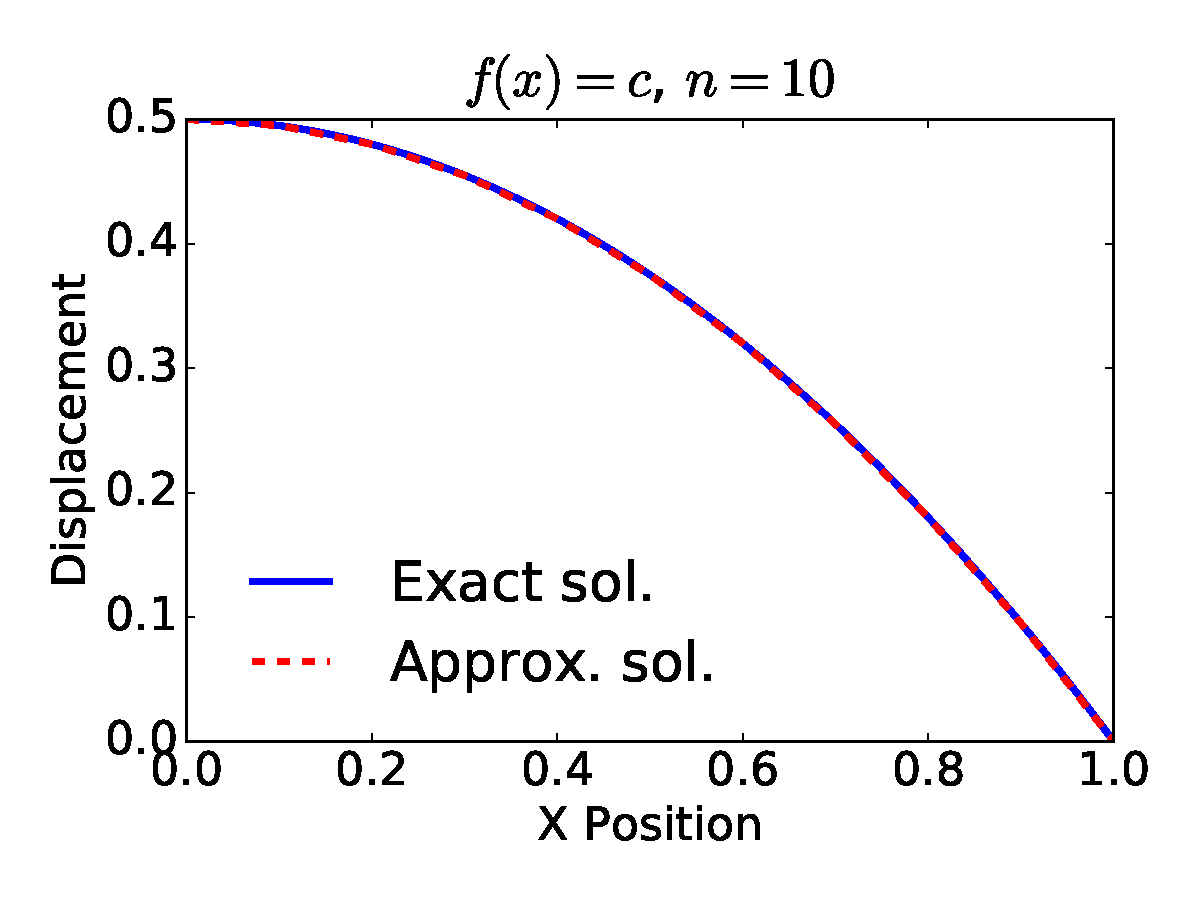
\includegraphics[width=\linewidth]{displacement_func0_Nell10}
                \label{fig:gull}
        \end{subfigure}%
        \begin{subfigure}[b]{0.33\textwidth}
                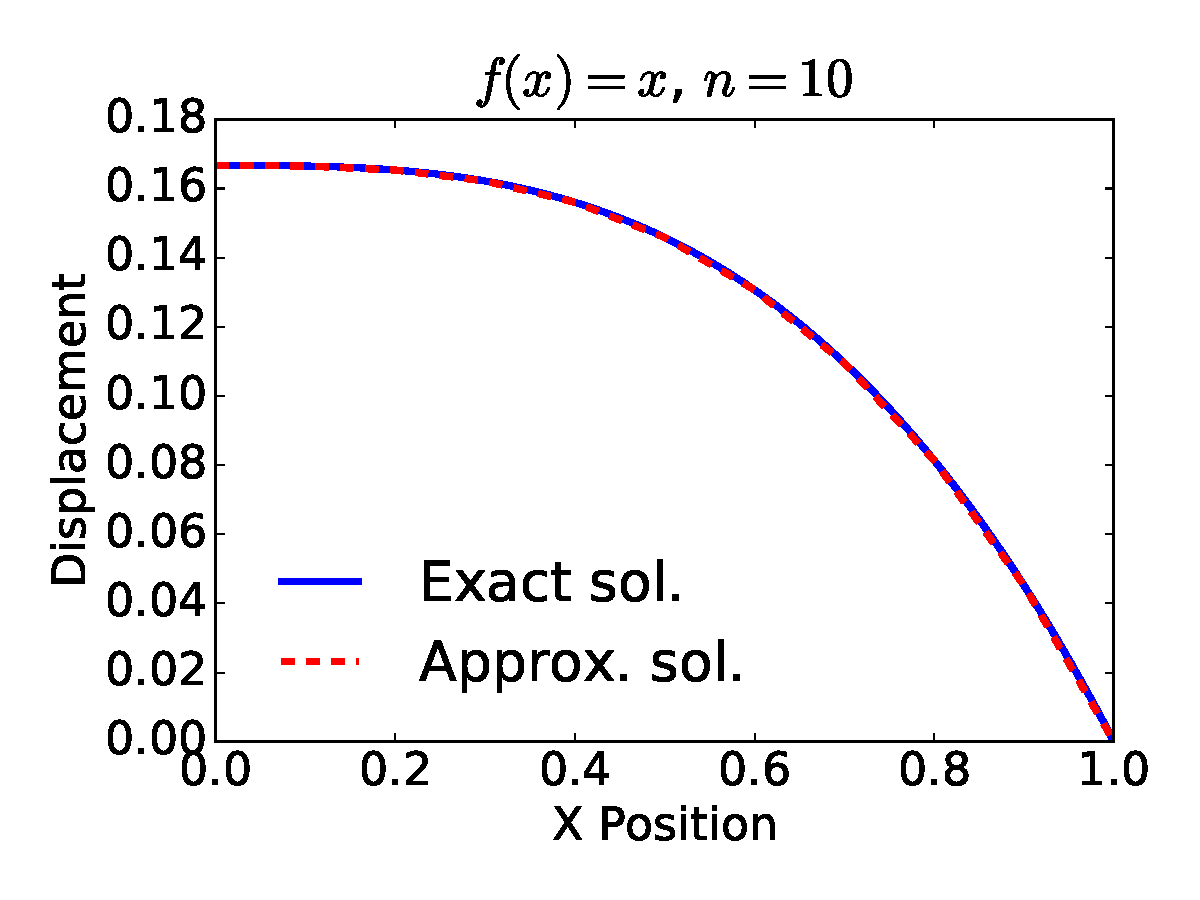
\includegraphics[width=\linewidth]{displacement_func1_Nell10}
                \label{fig:gull2}
        \end{subfigure}%
        \begin{subfigure}[b]{0.33\textwidth}
                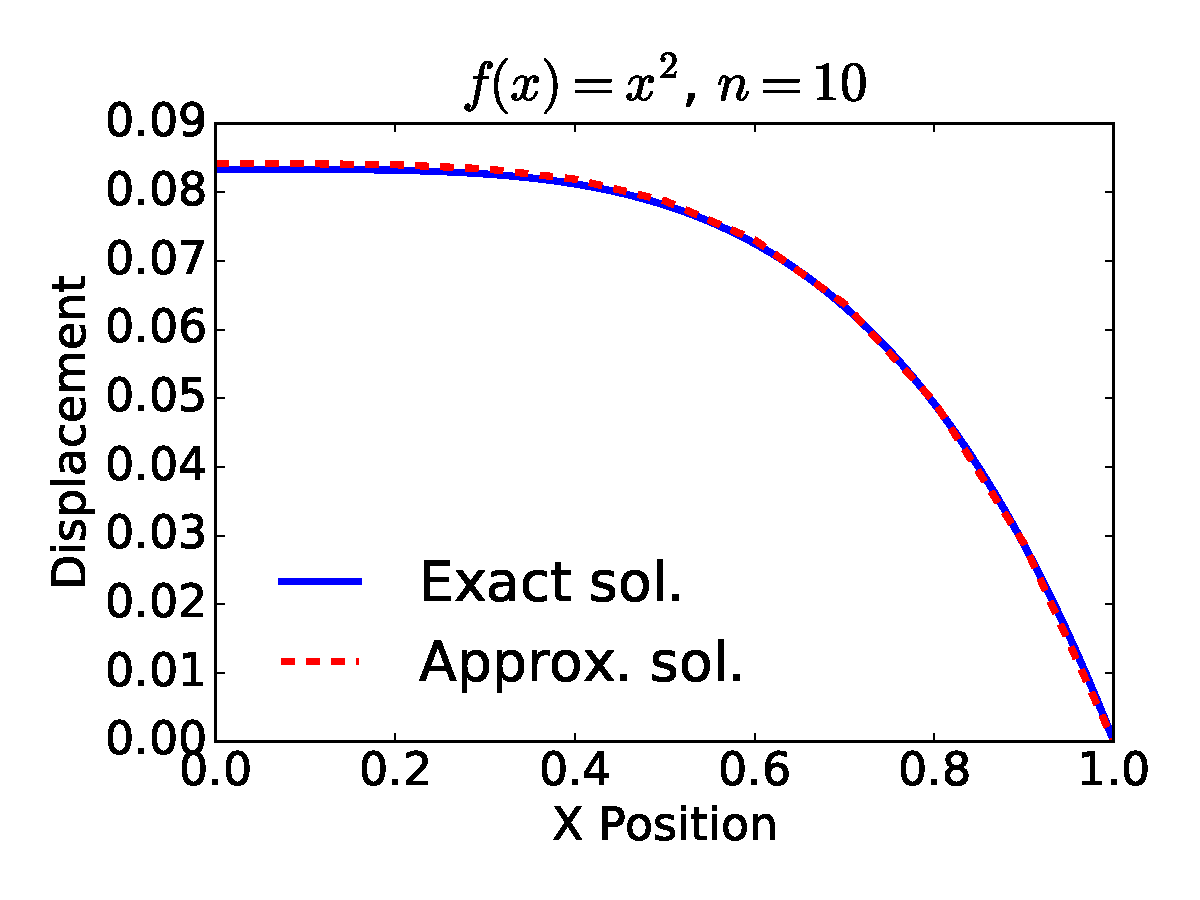
\includegraphics[width=\linewidth]{displacement_func2_Nell10}
                \label{fig:tiger}
        \end{subfigure}%
        
        \begin{subfigure}[b]{0.33\textwidth}
                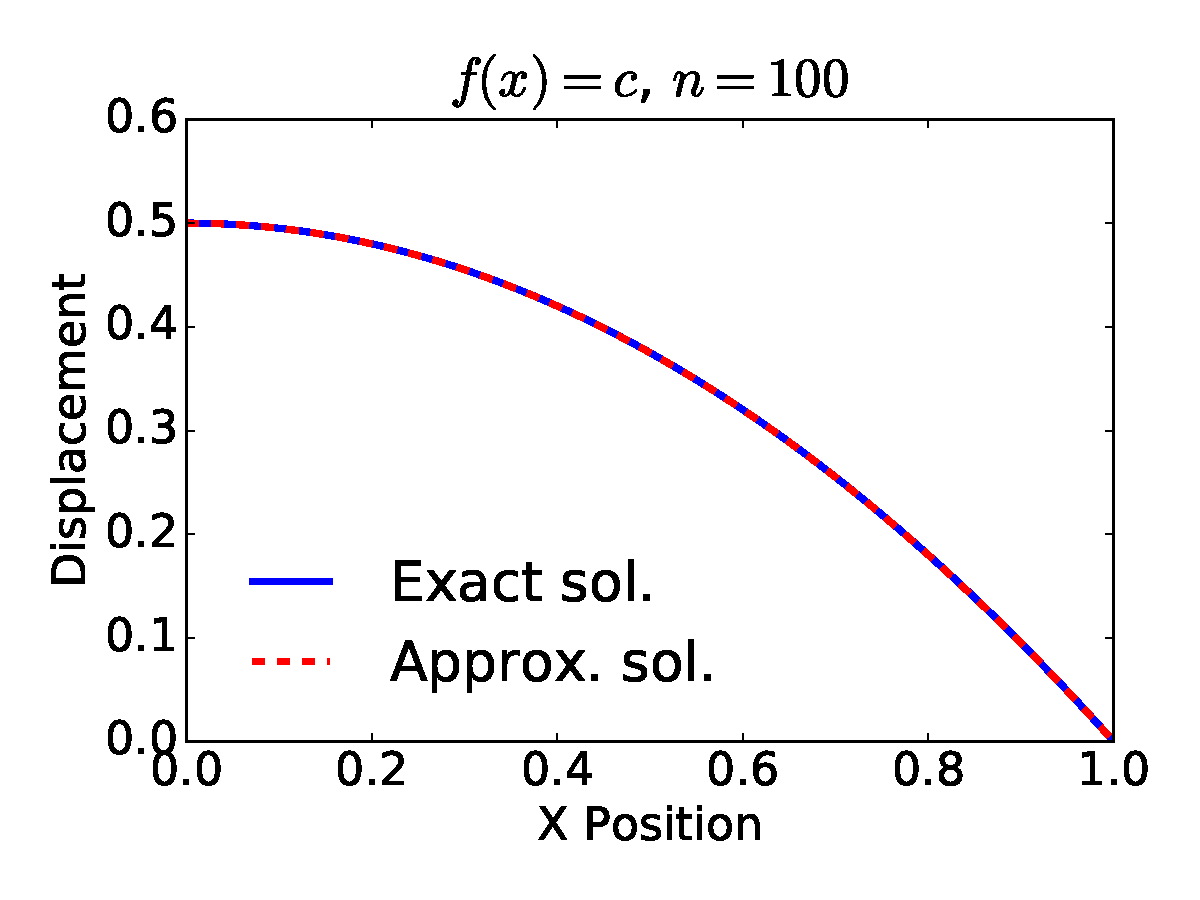
\includegraphics[width=\linewidth]{displacement_func0_Nell100}
                \label{fig:gull}
        \end{subfigure}%
        \begin{subfigure}[b]{0.33\textwidth}
                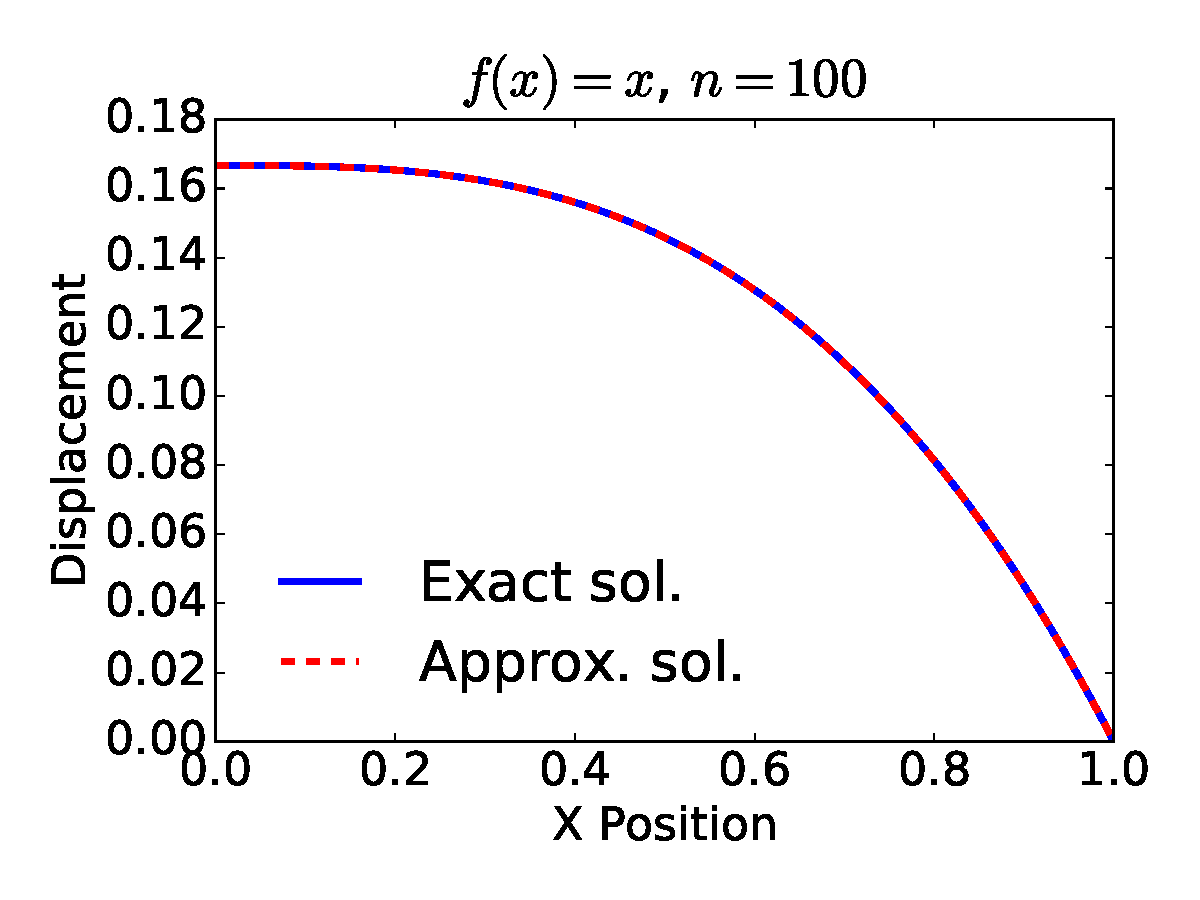
\includegraphics[width=\linewidth]{displacement_func1_Nell100}
                \label{fig:gull2}
        \end{subfigure}%
        \begin{subfigure}[b]{0.33\textwidth}
                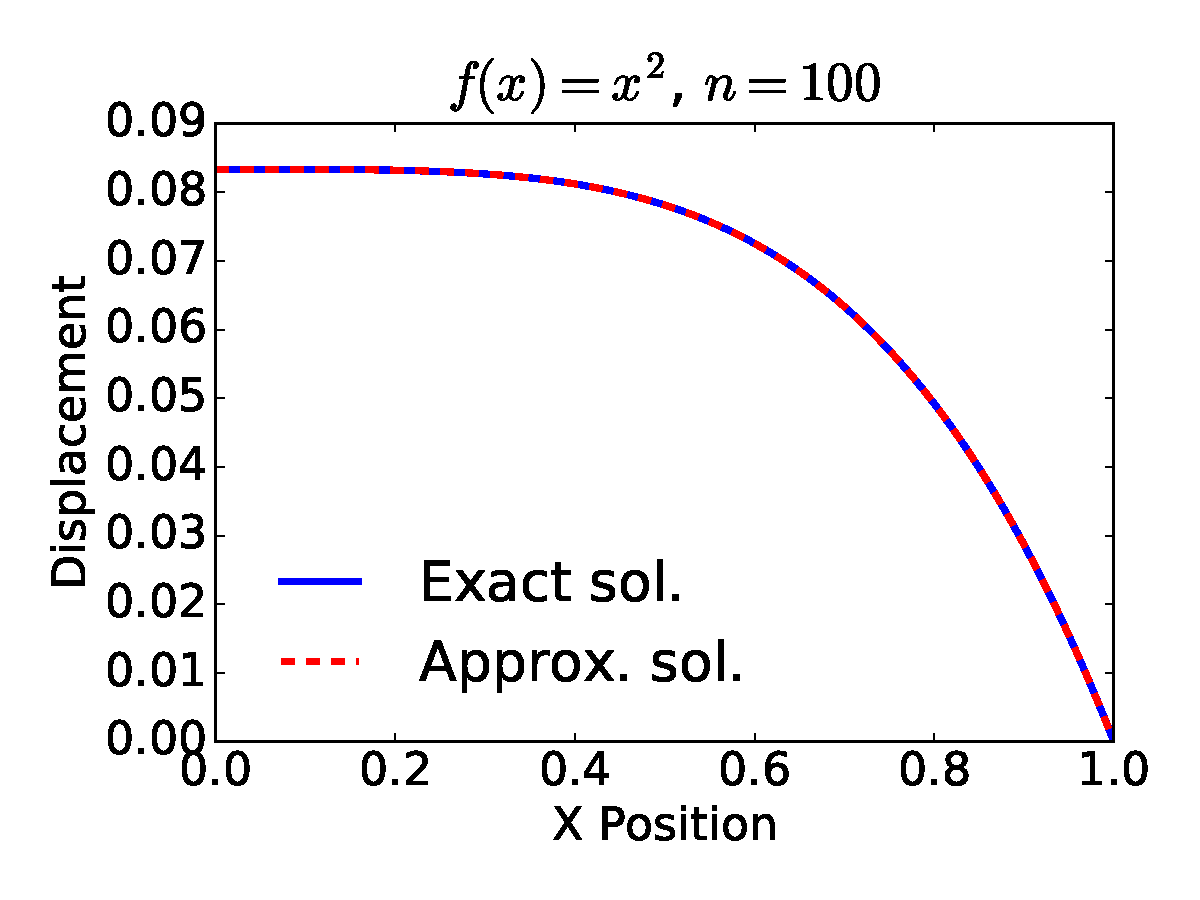
\includegraphics[width=\linewidth]{displacement_func2_Nell100}
                \label{fig:tiger}
        \end{subfigure}%
        
        \begin{subfigure}[b]{0.33\textwidth}
                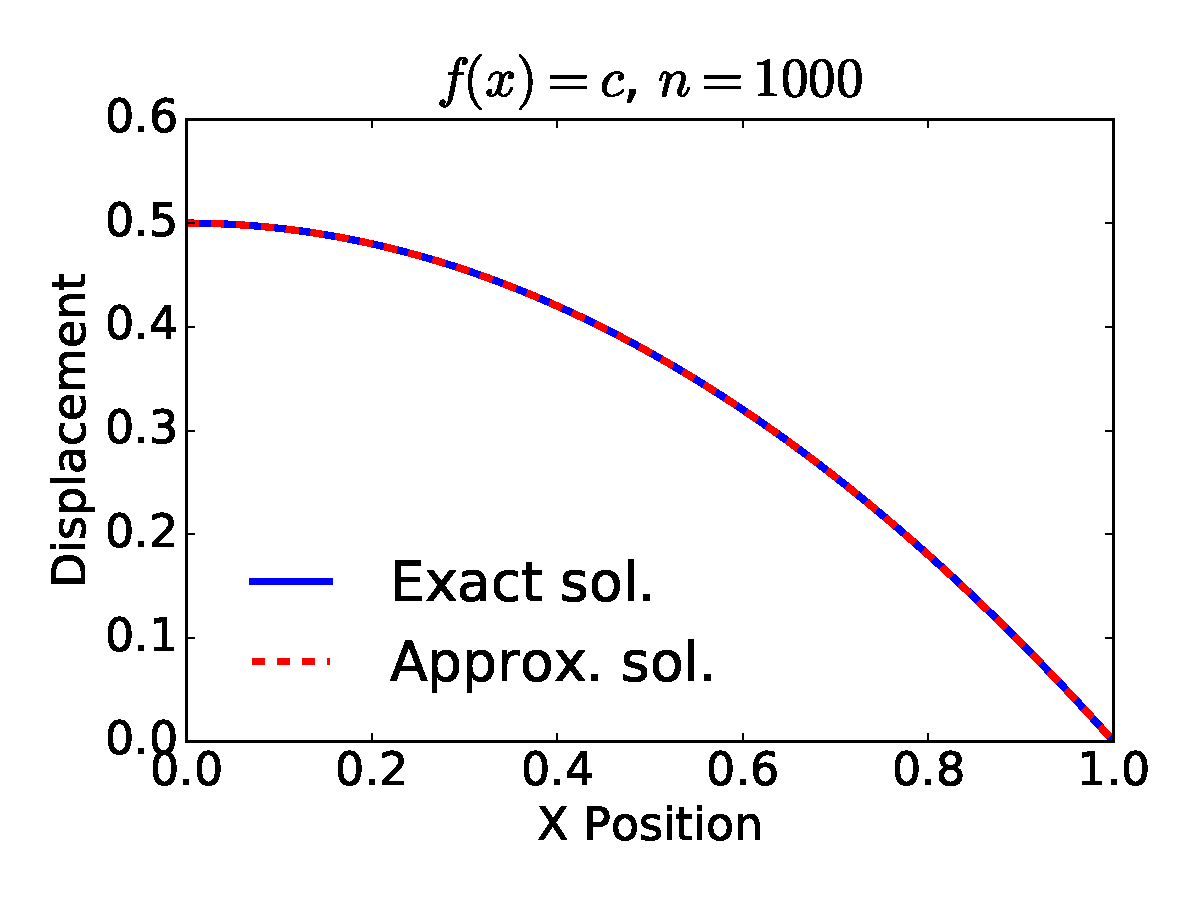
\includegraphics[width=\linewidth]{displacement_func0_Nell1000}
                \label{fig:gull}
        \end{subfigure}%
        \begin{subfigure}[b]{0.33\textwidth}
                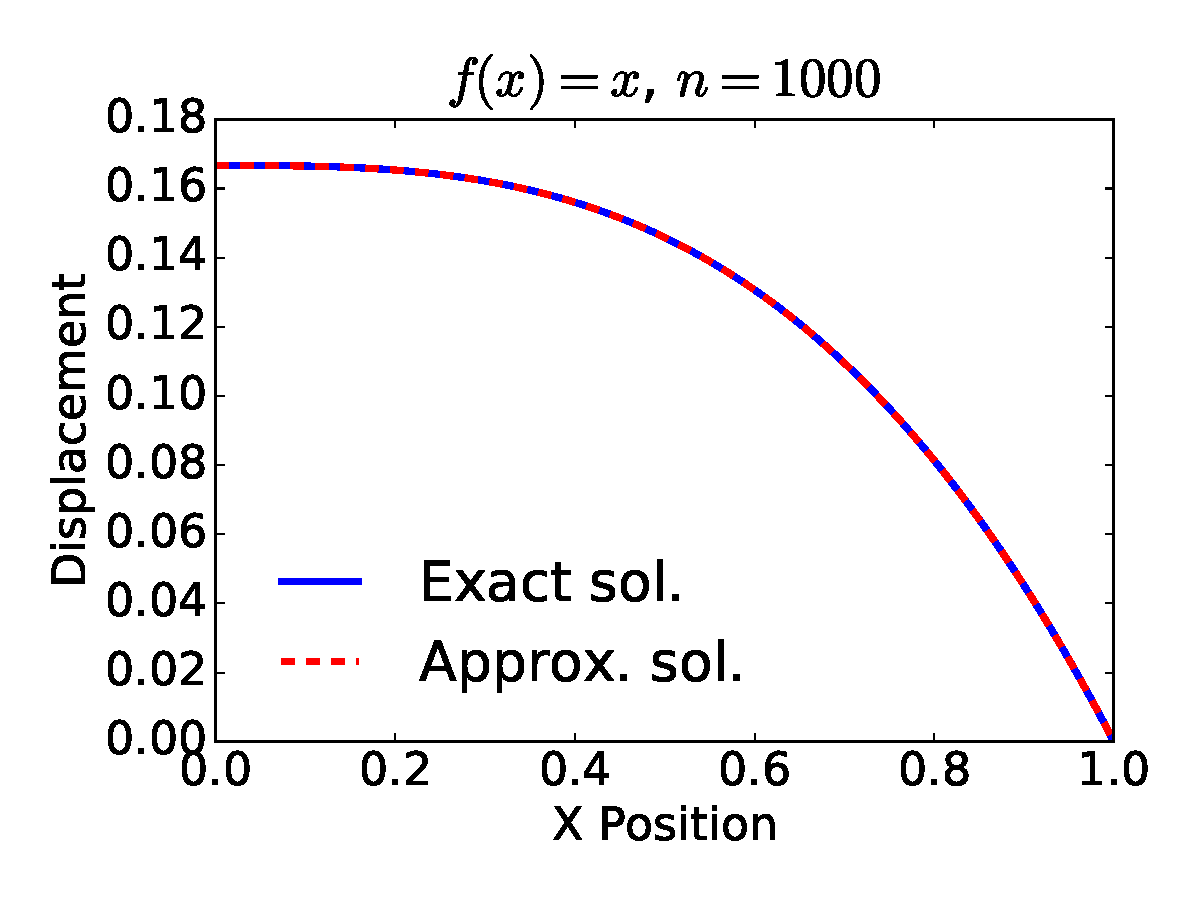
\includegraphics[width=\linewidth]{displacement_func1_Nell1000}
                \label{fig:gull2}
        \end{subfigure}%
        \begin{subfigure}[b]{0.33\textwidth}
                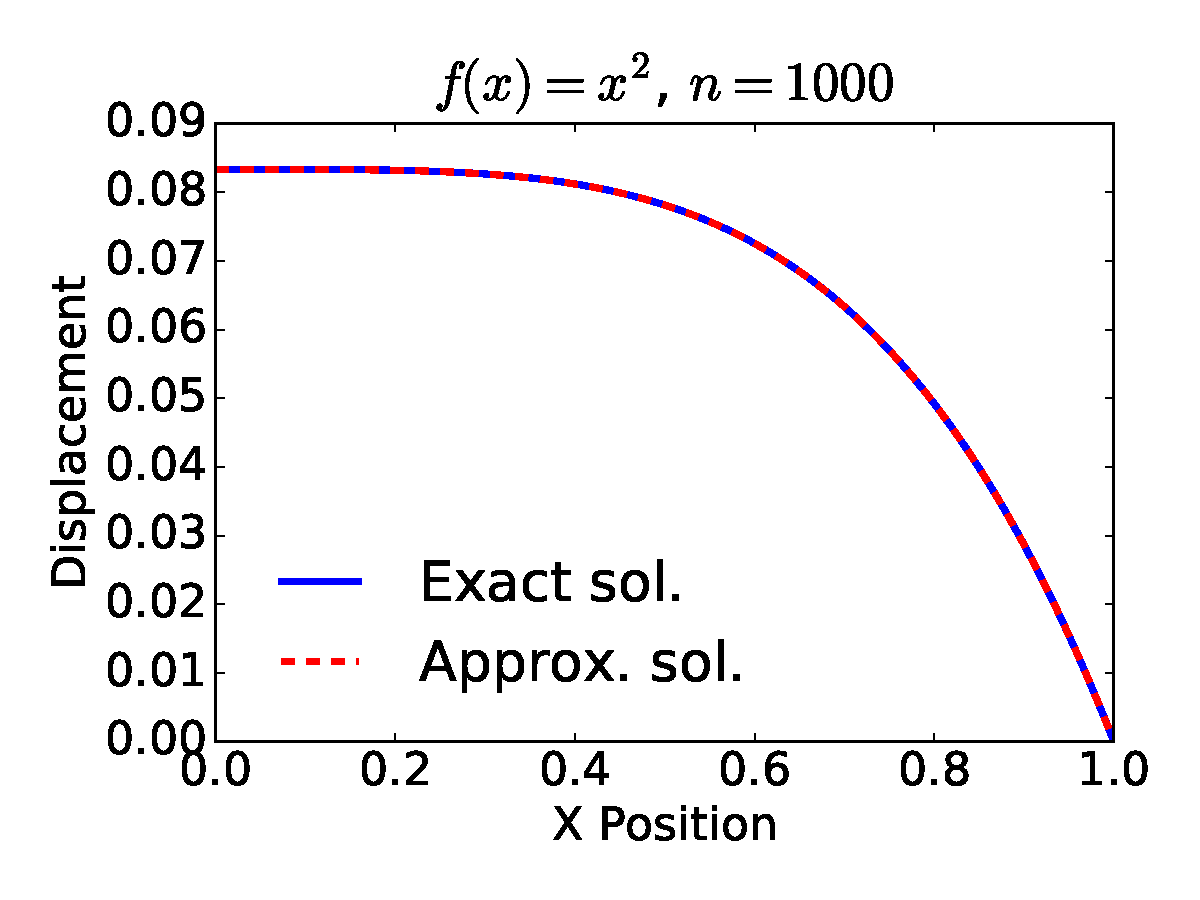
\includegraphics[width=\linewidth]{displacement_func2_Nell1000}
                \label{fig:tiger}
        \end{subfigure}%
        
        \begin{subfigure}[b]{0.33\textwidth}
                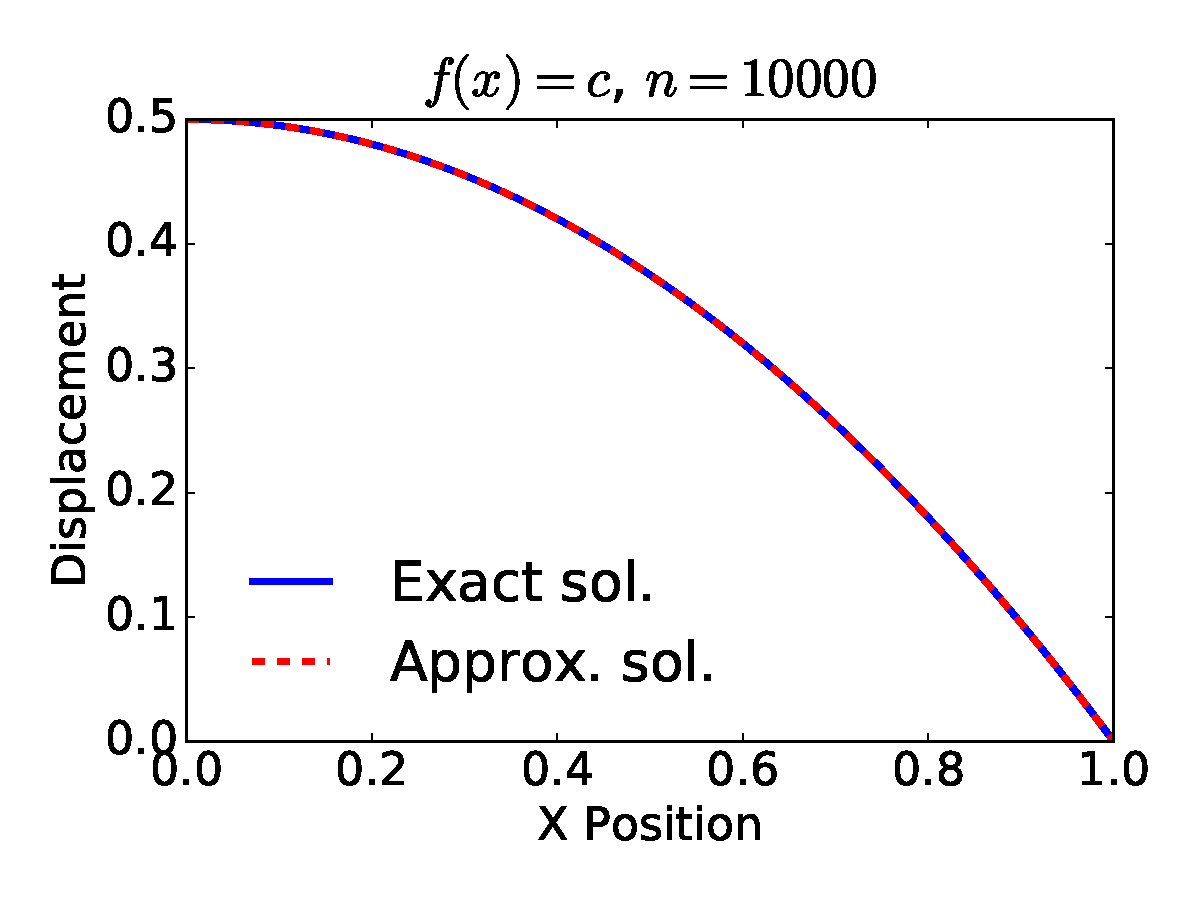
\includegraphics[width=\linewidth]{displacement_func0_Nell10000}
                \label{fig:gull}
        \end{subfigure}%
        \begin{subfigure}[b]{0.33\textwidth}
                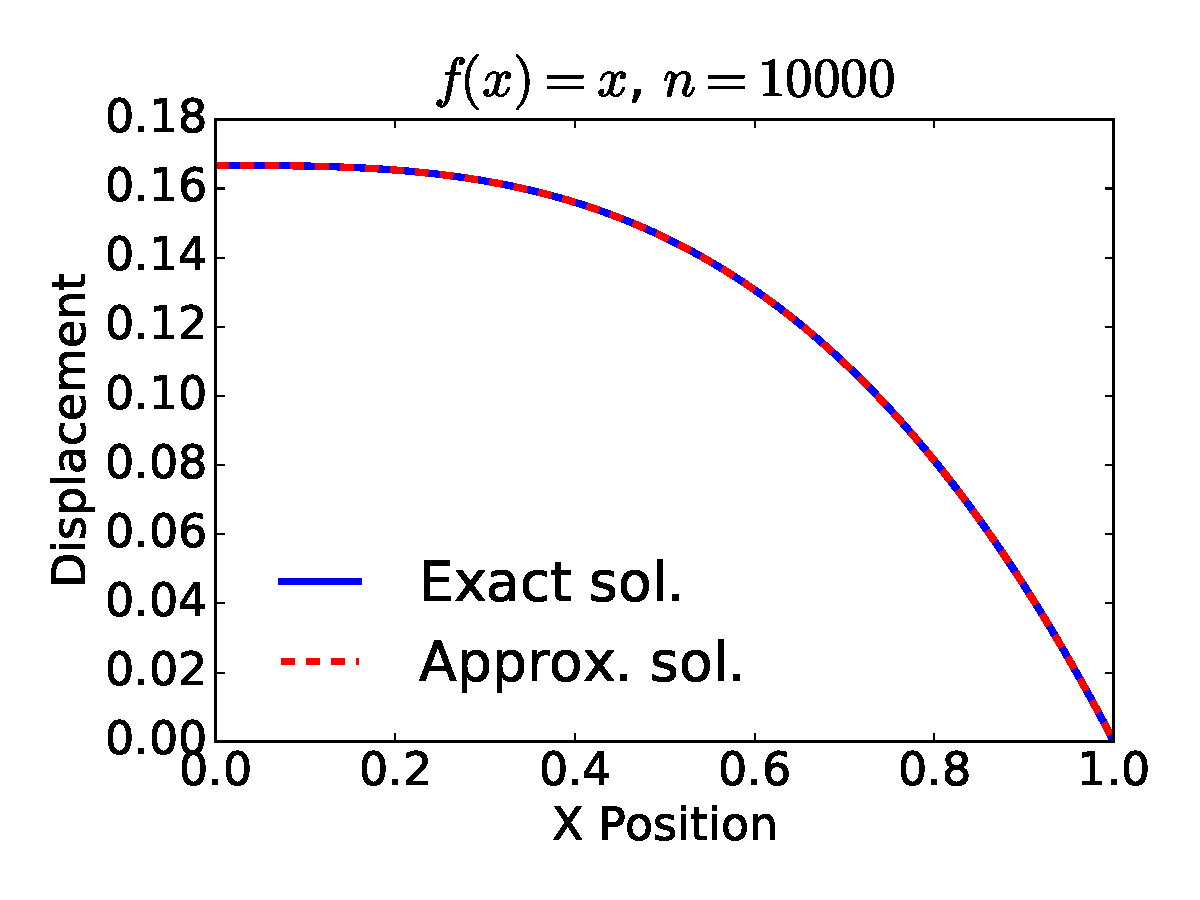
\includegraphics[width=\linewidth]{displacement_func1_Nell10000}
                \label{fig:gull2}
        \end{subfigure}%
        \begin{subfigure}[b]{0.33\textwidth}
                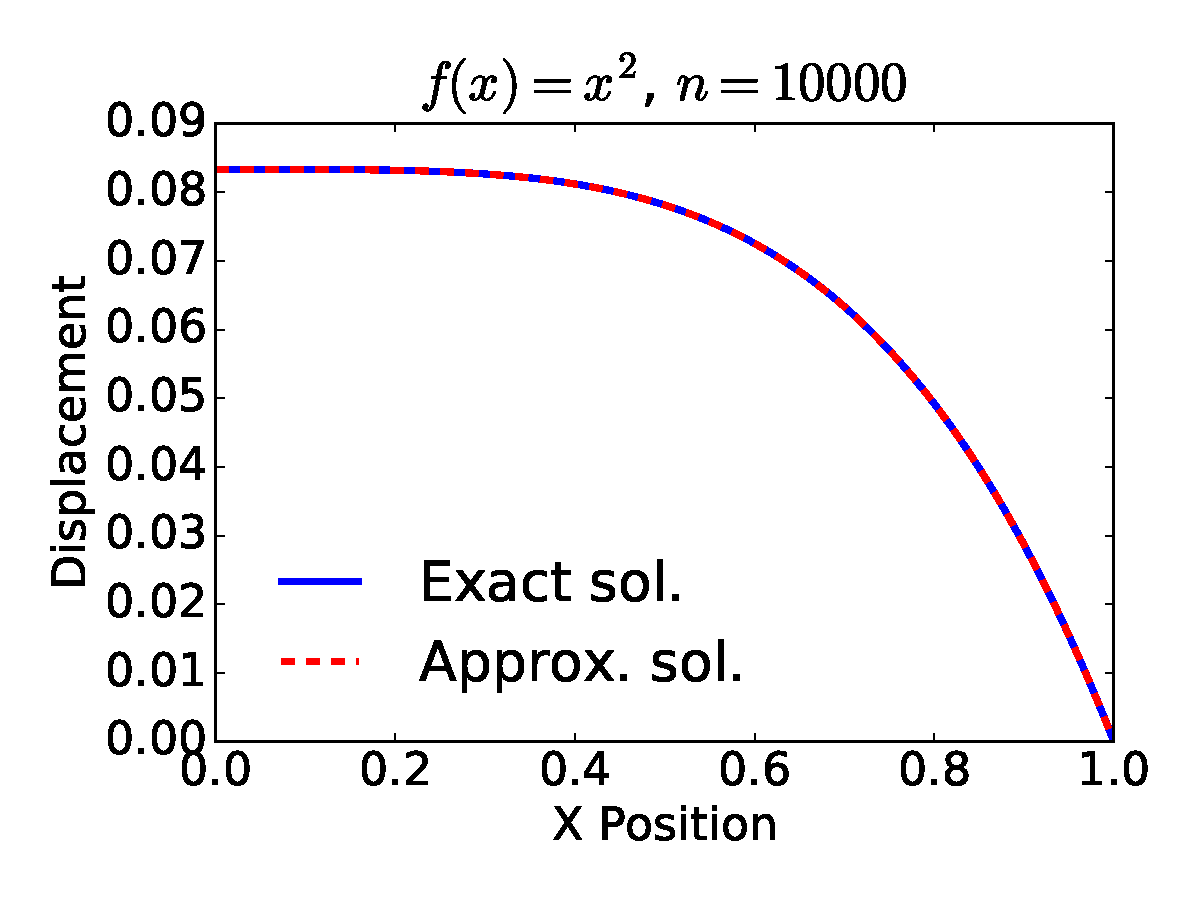
\includegraphics[width=\linewidth]{displacement_func2_Nell10000}
                \label{fig:tiger}
        \end{subfigure}%
        \caption{Exact and approximate solutions for each $f(x)$ and $n$}\label{fig:fandn}
\end{figure}

The approximate solution is exact at the nodes for the constant and linear forcing functions because we are approximating using first order polynomials. However, for the second order polynomial forcing function, the solution is not even exact at the nodes because we are ignorming higher order terms in our approximation. For all the forcing functions, the approximation is closer to the exact solution at points closer to nodes and further from the exact solution at points further from the nodes.

\section{Compute and report the global error for each $f(x)$ and $n$ (12 numbers)}
\begin{tabular}{l | l l l}
N-elements              & $f(x)=c$ & $f(x)=x$ & $f(x)=x^2$ \\
\hline
10 & 9.128709291753452602e-04 & 5.264090438827071818e-04& 5.908095390718911578e-04 \\
100 & 9.128709291329707023e-06 & 5.270399081649309119e-06 & 5.931474041855632921e-06  \\
1,000  & 9.128709226791299245e-08 & 5.270462112780296755e-08 & 5.931707788287919871e-08          \\
10,000     & 9.129188732190131811e-10 & 5.270659276938995368e-10 & 5.931669081979712336e-10  \\
\end{tabular}

\section{Employing the data for n = 10, 100, 1000, 10000 generate a log-log plot for $e$ versus $h$ for each $f(x)$ (1 plot). Determine the slope of the graph for the two cases when $f(x)$ is non-constant. The slope of this graph is the rate of convergence of the method or how fast the approximate solution is converging to the exact solution as the mesh is refined. How does the rate of convergence depend on $n$?}

Please see the error plot in \cref{fig:error}. The slope of the graph in loglog space is 1.99981946665 when $f(x)=x$ and 1.99942352808 when $f(x)=x^2$. The rate of convergence decreases as $n$ increases. This means that there are diminisiong returns in accuracy for increasing the number of elements.

\begin{figure}
	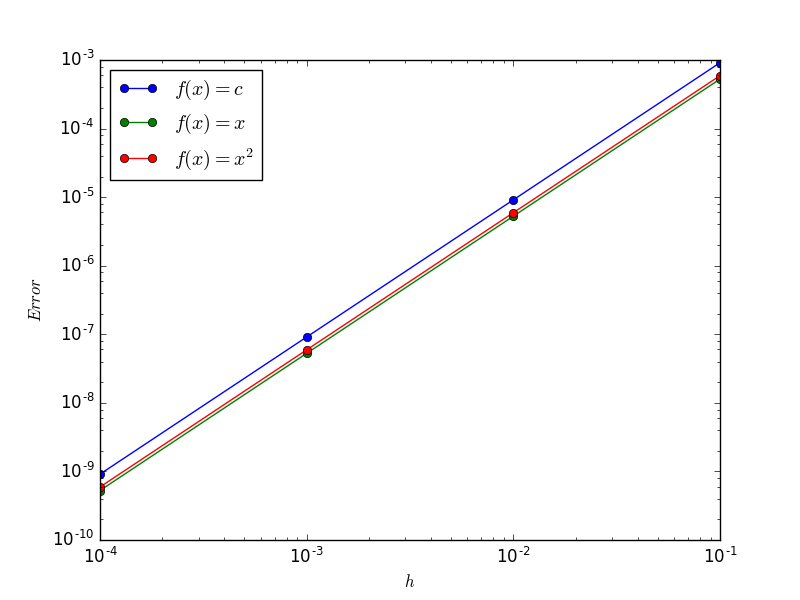
\includegraphics{error}
	\caption{Error plot for each $f(x)$ and $n$}\label{fig:error}
\end{figure}
\end{document}